\documentclass{beamer}
 
\usepackage[utf8]{inputenc}

\usetheme{Madrid}
\usecolortheme{default}

\usepackage[qm]{qcircuit}
\usepackage{bibentry}













\usepackage{physics}
\usepackage{amsmath}
\usepackage{amsfonts}
\usepackage{esint}
\usepackage{bbold}
\usepackage{mathtools}
\usepackage{dsfont}
\usepackage{amsthm}
\usepackage{bbm}
\usepackage{amssymb}
\theoremstyle{definition}
\newtheorem{defn}{Definition}[section]
\newtheorem{prop}{Properties}[section]
\newtheorem{rmk}{Remark}[section]
\newtheorem{exmp}{Example}[section]
\newtheorem{prob}{Problem}[section]
\newtheorem{sln}{Solution}[section]
\newtheorem{thm}{Theorem}[section]
\newtheorem*{prob*}{Problem}
\newtheorem*{sln*}{Solution}
\usepackage{empheq}
\usepackage{tensor}
\usepackage{hyperref}
\usepackage{xcolor}

\newcommand{\R}{\mathbb{R}}
\newcommand{\F}{\mathcal{F}}
\newcommand{\p}{\partial}

\newcommand{\V}{\mathbf{V}}
\newcommand{\W}{\mathbf{W}}
\newcommand{\Z}{\mathbf{Z}}
\newcommand{\Y}{\mathbf{Y}}
\newcommand{\U}{\mathbf{U}}
\newcommand{\X}{\mathbf{X}}

\newcommand{\A}{\mathcal{A}}
\newcommand{\B}{\mathcal{B}}

\newcommand{\xpan}{\text{span}}

\newcommand{\lag}{\mathcal{L}}

\newcommand{\J}{\mathbf{J}}

\newcommand{\M}{\mathcal{M}}

\newcommand{\K}{\mathcal{K}}

\newcommand{\N}{\mathcal{N}}

\newcommand{\E}{\mathcal{E}}

\newcommand{\ima}{\text{Im}}
\newcommand{\lin}{\overset{\text{linear}}{\longrightarrow}}
\newcommand{\T}{\mathcal{T}}
\newcommand{\poly}{\mathbb{P}}
\newcommand{\s}{\mathcal{S}}

\newcommand{\gives}{\rotatebox[origin=c]{180}{$\Rsh$}	}


\newcommand{\bigzero}{\mbox{\normalfont\Large\bfseries 0}}
\newcommand{\rvline}{\hspace*{-\arraycolsep}\vline\hspace*{-\arraycolsep}}




 
 
%Information to be included in the title page:
\title{Matrix Theory in a 2-Qubit Entangler}
\author[Huan Q. Bui] % (optional)
{Huan Q. Bui}

\institute[Colby College] % (optional)
{
	
	Matrix Analysis
	\and
	Professor Leo Livshits
}
\date{CLAS, May 2, 2019}
 
%\logo{
\includegraphics[height=0.3cm]{colby.png}}
 
\begin{document}
 
\frame{\titlepage}
 
\begin{frame}
\frametitle{Presentation layout}
\tableofcontents
\end{frame}

\section{Qubits \& Quantum Gates}

\begin{frame}
\frametitle{Qubits \& Quantum Gates}
\textit{Qubit:} A quantum system with two measurable physical states $\ket{0}$ and $\ket{1}$,
\begin{align*}
\ket{0} = \begin{bmatrix}
1\\0
\end{bmatrix}\hspace{0.5cm} \ket{1} = \begin{bmatrix}
0\\1
\end{bmatrix}.
\end{align*}
Before measurement,
\begin{align*}
\ket{\psi} = a\ket{0} + b\ket{1} \in \mathbb{C}^2,\hspace{0.5cm} \abs{a}^2 + \abs{b}^2 = 1.
\end{align*}

Physically,
\begin{align*}
P(\ket{\psi} \to \ket{0}) = \abs{a}^2\hspace{0.5cm}
P(\ket{\psi} \to \ket{1}) = \abs{b}^2.
\end{align*}

\textit{Quantum gate:} a unitary transformation on $\ket{\psi}$. 
\end{frame}

\begin{frame}
\frametitle{Qubits \& Quantum Gates}

\textit{Multiple Qubits}: States of $k$ qubits is a vector in $\otimes^k\mathbb{C}^2$ with basis vectors
\begin{align*}
\ket{x_1\dots x_k} = \ket{x_1}\otimes \dots \otimes \ket{x_k}, \hspace{0.5cm} x_i \in \{0,1\}.
\end{align*}
``$\otimes$'': Kronecker product. If $\A \in \mathbb{M}_{m\times n}$ and $\B \in \mathbb{M}_{p\times q}$, then
\begin{align*}
\A \otimes \B = \begin{bmatrix}
a_{11}\B & \dots & a_{1n}\B\\
\vdots & \ddots & \vdots\\
a_{m1}\B & \dots & a_{mn}\B
\end{bmatrix}.
\end{align*}
\end{frame}

\begin{frame}
\frametitle{Kronecker Products}
\underline{Example}: Representing the classical numbers ``1'' and ``0'' with two qubits:
\begin{align*}
&1_2 \equiv \ket{01} = \ket{0} \otimes \ket{1} = \begin{bmatrix}
1\\0
\end{bmatrix}\otimes 
\begin{bmatrix}
0\\1
\end{bmatrix}
=
\begin{bmatrix}
1\begin{bmatrix}
0\\1
\end{bmatrix}\\
0\begin{bmatrix}
0\\1
\end{bmatrix}
\end{bmatrix} = \begin{bmatrix}
0\\1\\0\\0
\end{bmatrix}\\
&0_2 \equiv \ket{00} = \ket{0} \otimes \ket{0} = \begin{bmatrix}
1\\0
\end{bmatrix}\otimes 
\begin{bmatrix}
1\\0
\end{bmatrix}
=
\begin{bmatrix}
1\begin{bmatrix}
1\\0
\end{bmatrix}\\
0\begin{bmatrix}
1\\0
\end{bmatrix}
\end{bmatrix} = \begin{bmatrix}
1\\0\\0\\0
\end{bmatrix}\\
&\hspace{0.5cm}\ket{10} = \begin{bmatrix}
0&0&1&0
\end{bmatrix}^\top, \ket{11} = \begin{bmatrix}
0&0&0&1
\end{bmatrix}^\top.
\end{align*}
In fact, $\ket{00}, \ket{01}, \ket{10}, \ket{11}$ form a basis for $\otimes^2\mathbb{C}^{2}$, the 2-qubit system.
\end{frame}

\begin{frame}
\frametitle{Kronecker Products}
Doesn't care where scalar goes...
$$ (\alpha \A) \otimes \B = \A \otimes (\alpha \B) = \alpha(\A \otimes \B)$$
Associative: $$(\A \otimes \B) \otimes \mathcal{C} = \A \otimes (\B \otimes \mathcal{C})$$
Left-distributive: $$\A \otimes (\B + \mathcal{C}) = \A\otimes \B + \A \otimes \mathcal{C}$$
Right-distributive: $$(\A + \B)\otimes \mathcal{C} = \A \otimes \mathcal{B} + \B \otimes \mathcal{C}$$
\end{frame}

\begin{frame}
\frametitle{Tensor Products}
hello
\end{frame}

\begin{frame}
\frametitle{Quantum Gates}
\textit{Quantum Gates}: Represented by unitary matrices $\rightarrow$ Reversible. Act on spaces of one or many qubits. Example: 
\begin{align*}
Hadamard: H = \frac{1}{\sqrt{2}}\begin{bmatrix}
1&1\\1&-1
\end{bmatrix}, \hspace{0.5cm}
CNOT_1 = \begin{bmatrix}
1&0&0&0\\
0&1&0&0\\
0&0&0&1\\
0&0&1&0
\end{bmatrix}
\end{align*}

\textit{Measurements}: Irreversible $\rightarrow$ Not quantum gates.
\end{frame}


\begin{frame}
\frametitle{Multi-qubit systems}

\begin{itemize}

\item Representing a multi-qubit state as many single-qubit states?
\item Representing a multi-qubit gate as many single-qubit gates?
\end{itemize}
\end{frame}



\begin{frame}
\frametitle{Recipe}

What do we need to entangle two qubits?
\begin{itemize}
	\item Tensor products
	\item Hadamard gate
	\item CNOT gate
	\item Measure
\end{itemize}
\end{frame}








\section{Some Matrix Theory}

\begin{frame}
\frametitle{Tensor Products}
The \textit{tensor product} of $\V = \mathbb{C}^{\Sigma_1}$ and $\W = \mathbb{C}^{\Sigma_2}$ is
\begin{align*}
\V \otimes \W = \mathbb{C}^{\Sigma_1 \times \Sigma_2}.
\end{align*}
\textit{Elementary tensors} span $\V\otimes \W$. For $\ket{v} \in \V$ and $\ket{w} \in \W$, 
\begin{align*}
\ket{v}\otimes \ket{w}\equiv \ket{v}\ket{w} \equiv \ket{vw}  \in \V \otimes \W.
\end{align*} 

\underline{Example}: Representing the classical number ``1'' with two qubits:
\begin{align*}
1_2 \equiv \ket{01} = \ket{0} \otimes \ket{1} = \begin{bmatrix}
1\\0
\end{bmatrix}\otimes 
\begin{bmatrix}
0\\1
\end{bmatrix}
=
\begin{bmatrix}
1\begin{bmatrix}
0\\1
\end{bmatrix}\\
0\begin{bmatrix}
0\\1
\end{bmatrix}
\end{bmatrix} = \begin{bmatrix}
0\\1\\0\\0
\end{bmatrix}.
\end{align*}


\end{frame}











\begin{frame}
\frametitle{Tensor Products (cont.)}

$\xpan(\ket{00}, \ket{01}, \ket{10}, \ket{11}) = \V\otimes \W$, where
\begin{align*}
\ket{00} = \begin{bmatrix}
1&0&0&0
\end{bmatrix}^\top, \ket{10} = \begin{bmatrix}
0&0&1&0
\end{bmatrix}^\top, \ket{11} = \begin{bmatrix}
0&0&0&1
\end{bmatrix}^\top.
\end{align*}
Linear independence $\rightarrow$ $(\ket{00}, \ket{01}, \ket{10}, \ket{11})$ form a computational basis. \\
$\,$\\
A \textit{generic state}: For $\abs{a_{00}}^2 + \abs{a_{01}}^2 + \abs{a_{10}}^2 + \abs{a_{11}}^2 = 1$,
\begin{align*}
\ket{\psi} = a_{00}\ket{00} + a_{01}\ket{01} + a_{10}\ket{10} + a_{11}\ket{11}.
\end{align*}

\end{frame}


\begin{frame}
\frametitle{Tensor Products (cont.)}
Not every $\ket{\psi} \in \V\otimes \W$ is an elementary tensor. \\
$\,$\\
\underline{Example}: There are no states $\ket{c}, \ket{d} \in \mathbb{C}^2$ such that
\begin{align*}
\ket{c} \otimes \ket{d} = \ket{\beta_{00}} &= \begin{bmatrix}
\frac{1}{\sqrt{2}} & 0 & 0 & \frac{1}{\sqrt{2}}
\end{bmatrix}^\top \\
&= \frac{1}{\sqrt{2}}\ket{00} + \frac{1}{\sqrt{2}}\ket{11}
\end{align*}
\underline{Examples}: Bell states
\begin{align*}
\ket{\beta_{10}} = \frac{1}{\sqrt{2}}\ket{00} - \frac{1}{\sqrt{2}}\ket{11}\\
\ket{\beta_{01}} = \frac{1}{\sqrt{2}}\ket{01} + \frac{1}{\sqrt{2}}\ket{10}\\
\ket{\beta_{11}} = \frac{1}{\sqrt{2}}\ket{01} - \frac{1}{\sqrt{2}}\ket{10}\\
\end{align*}
\end{frame}

\begin{frame}
\frametitle{Tensor Products (cont.)}
\textit{For operators:} $\A \in \mathfrak{\lag}(\V), \mathcal{B} \in \mathfrak{\lag}(\W)$, $\A\otimes \B \in \mathfrak{\lag}(\V \otimes \W)$ is defined by
\begin{align*}
(\A \otimes \B)(\ket{v}\otimes \ket{w}) = (\A\ket{v})\otimes (\B\ket{w}).
\end{align*}
Not all $C \in \mathfrak{\lag}(\V\otimes \W)$ can be written as $\A \otimes \B$, $\A \in \mathfrak{\lag}(\V), \mathcal{B} \in \mathfrak{\lag}(\W)$.\\
$\,$\\
\underline{Example}:
\begin{align*}
CNOT_1 = \begin{bmatrix}
1&0&0&0\\
0&1&0&0\\
0&0&0&1\\
0&0&1&0
\end{bmatrix} 
\hspace{0.5cm}
SWAP = 
\begin{bmatrix}
1&0&0&0\\
0&0&1&0\\
0&1&0&0\\
0&0&0&1
\end{bmatrix} 
\end{align*}
\end{frame}


\begin{frame}
\frametitle{$SWAP \neq S_1 \otimes S_2$}
Consider the 2-qubit $SWAP$ map:
\begin{align*}
SWAP = 
\begin{bmatrix}
1&0&0&0\\
0&0&1&0\\
0&1&0&0\\
0&0&0&1
\end{bmatrix} \in \lag(\V\otimes \W).
\end{align*}
Observe: 
\begin{align*}
SWAP(\ket{0}\otimes \ket{1}) = \ket{1}\otimes \ket{0}.
\end{align*}
Suppose for $S_1 \in \lag(\V), S_2 \in \lag(\W)$
\begin{align*}
SWAP = S_1 \otimes S_2
\end{align*}
\end{frame}


\begin{frame}
\frametitle{Example: 2-Qubit Entanglement Circuit}
\begin{center}
	$\,$\Qcircuit @C=.7em @R=.4em  {
		\lstick{a: \ket{0}} & \qw & \qw & \targ & \meter & \qw \\
		\lstick{b: \ket{0}} & \qw & \gate{H} & \ctrl{-1}& \meter & \qw 
	}
\end{center}
\begin{align*}
H\begin{bmatrix}
1\\0
\end{bmatrix}_b = \frac{1}{\sqrt{2}}\begin{bmatrix}
1&1\\1&-1
\end{bmatrix}\begin{bmatrix}
1\\0
\end{bmatrix}_b = \frac{1}{\sqrt{2}}\ket{0}_b + \frac{1}{\sqrt{2}}\ket{1}_b
\end{align*}
\begin{align*}
CNOT_b = C_b = \begin{bmatrix}
1&0&0&0\\
0&0&0&1\\
0&0&1&0\\
0&1&0&0
\end{bmatrix}\hspace{0.5cm}
\begin{cases}
\ket{00} \to \ket{00}\\
\ket{10} \to \ket{10}\\
\ket{01} \to \ket{11}\\
\ket{11} \to \ket{01}
\end{cases}
\end{align*}
%$\rightarrow$ Unitary Operations $\equiv$ Quantum Gates
\end{frame}

\begin{frame}
\frametitle{Example: Entanglement (cont.)}
Notice:
\begin{align*}
(I\ket{0}) \otimes (H_b\ket{0}) &= (I \otimes H_b)(\ket{0} \otimes \ket{0}) \\
\begin{bmatrix}
1\\0
\end{bmatrix}
\otimes
\frac{1}{\sqrt{2}}
\begin{bmatrix}
1&1\\1&-1
\end{bmatrix}
\begin{bmatrix}
1\\0
\end{bmatrix}
&=
\begin{bmatrix}
\frac{1}{\sqrt{2}}\begin{bmatrix}
1&1\\
1&-1
\end{bmatrix}& \mathcal{O}\\
\mathcal{O} & \frac{1}{\sqrt{2}}\begin{bmatrix}
1&1\\1&-1
\end{bmatrix}
\end{bmatrix}\begin{bmatrix}
1\\0\\0\\0
\end{bmatrix}\\
\begin{bmatrix}
\frac{1}{\sqrt{2}} & \frac{1}{\sqrt{2}} & 0&0
\end{bmatrix}^\top &= \begin{bmatrix}\frac{1}{\sqrt{2}} & \frac{1}{\sqrt{2}} & 0&0
\end{bmatrix}^\top 
\end{align*}
$\rightarrow$ Possible to write $H$ as $I \otimes H_b$. Not possible for $CNOT_b$.
\end{frame}


\begin{frame}
\frametitle{Example: Entanglement (cont.)}
\begin{center}
	$\,$\Qcircuit @C=.7em @R=.4em  {
		\lstick{a: \ket{0}} & \qw & \qw & \targ & \meter & \qw \\
		\lstick{b: \ket{0}} & \qw & \gate{H} & \ctrl{-1}& \meter & \qw 
	}
\end{center}
\begin{align*}
C_b(I \otimes H)\left(\begin{bmatrix}
1\\0
\end{bmatrix}_a
\otimes
\begin{bmatrix}
1\\0
\end{bmatrix}_b
\right)
&= C_b\left(\begin{bmatrix}
1&0\\0&1
\end{bmatrix}\begin{bmatrix}
1\\0
\end{bmatrix}_a\otimes \frac{1}{\sqrt{2}}\begin{bmatrix}
1&1\\1&-1
\end{bmatrix}\begin{bmatrix}
1\\0
\end{bmatrix}_b\right)\\
&=
\begin{bmatrix}
1&0&0&0\\
0&0&0&1\\
0&0&1&0\\
0&1&0&0
\end{bmatrix}
\begin{bmatrix}
1/\sqrt{2}\\1/\sqrt{2}\\0\\0
\end{bmatrix}
= 
\begin{bmatrix}
1/\sqrt{2}\\0\\0\\1/\sqrt{2}
\end{bmatrix}\\ &= \frac{1}{\sqrt{2}}\ket{0}\otimes\ket{0} + \frac{1}{\sqrt{2}}\ket{1}\otimes\ket{1}\\
&\rightarrow \textbf{Entangled}
\end{align*}
\end{frame}






\begin{frame}
\frametitle{Tensor Products (cont.)}
Other properties:
\begin{itemize}
	\item Bilinear: linear in both arguments.
	\item Associative
	\item Distributive
	\item Not commutative
	\item $(\A \otimes \B)^\dagger = \A^\dagger \otimes \B^\dagger$.
	\item $\Tr(\A\otimes \B) = \Tr(\A)\cdot \Tr(\B)$.
	\item $\det(\A \otimes \B) = (\det(\A))^m\cdot \det(\B)^n$, where $m = \text{size}(\A), n =\text{size}(\B)$. 
\end{itemize}
\end{frame}















\section{Simulation on IBM-Q}

\begin{frame}
\frametitle{Simulation on IBM-Q}

Entanglement circuit, revisited

\begin{center}
	$\,$\Qcircuit @C=.7em @R=.4em  {
		\lstick{a: \ket{0}} & \qw & \qw & \targ & \meter & \qw \\
		\lstick{b: \ket{0}} & \qw & \gate{H} & \ctrl{-1}& \meter & \qw 
	}

\begin{figure}[h!]
	\centering
	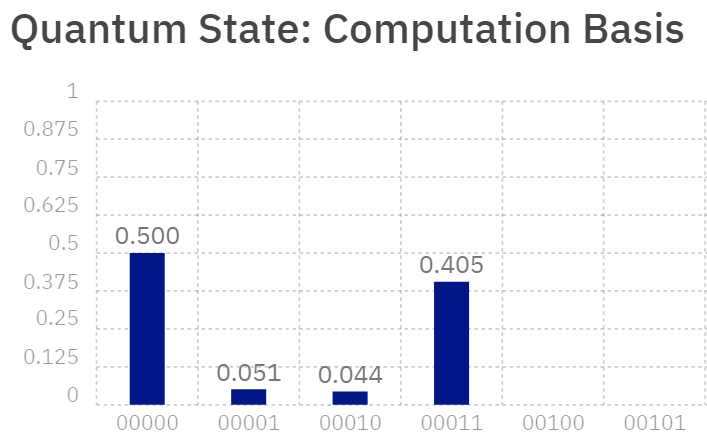
\includegraphics[scale=0.7]{ibmq}
\end{figure}
\end{center}


\end{frame}















\section{Recap}

\begin{frame}
\frametitle{Recap}

\begin{itemize}
	\item Representing multi-qubit systems with tensor products.
	\item Representing multi-qubit operators with tensor products.
	\item Not all multi-qubit states are a tensor product of 1-qubit states.
	\item Not all multi-qubit gates are a tensor product of 1-qubit gates.
	\item Entanglement on IBM-Q.
\end{itemize}

\end{frame}

\begin{frame}
\frametitle{References}



\bibliographystyle{amsalpha}
\bibliography{references}{}



\end{frame}



 
\end{document}
